\documentclass{article}

\usepackage{listings}
\usepackage{graphicx}
\usepackage{float}
\usepackage{amsmath}
\usepackage{geometry}
 \geometry{
 a4paper,
 total={170mm,257mm},
 left=20mm,
 top=20mm,
 }



\author{David Kolden, davidko}
\title{Mandatory assignment 1: Traveling Salesman Problem [INF4490]}

\begin{document}

\maketitle
\tableofcontents

\section{Introduction}
This report documents the results of implementing different algorithms to solve the 'Traveling salesman problem'. Four different algorithms are tested: exhaustive search, hill climbing, a genetic algorithm and a hybrid algorithm using elements from the genetic- and the hill climbing algorithm.

All the algorithms are more or less inspired by the examples and pseudo codes in \cite{eiben} and \cite{marsland}
 
\section{Exhaustive search}

This algorithm was made based on \cite[chapter 9.4.1]{marsland}. The program ineffectively searches every permutation of the number of cities, which means it searches permutations that in reality represents the same distances ([1, 2, 3], [2, 3, 1], [3, 2, 1], etc.)

Start the program
\begin{lstlisting}[language=bash]
	$ python3 exhaustive.py european_cities.csv 
\end{lstlisting}
The program will find the shortest tour between 6 - 10 cities. The program outputs

\begin{lstlisting}[language=bash]
	For n_cities = 6:
	Best distance: 5018.8099999999995
	Best sequence: (0, 1, 4, 5, 2, 3)
	Best order of travel: Barcelona Belgrade Bucharest Budapest Berlin 
	Brussels Barcelona
 
	For n_cities = 7:
	Best distance: 5487.889999999999
	Best sequence: (2, 6, 3, 0, 1, 4, 5)
	Best order of travel: Berlin Copenhagen Brussels Barcelona Belgrade 
	Bucharest Budapest Berlin
 
	For n_cities = 8:
	Best distance: 6667.489999999999
	Best sequence: (3, 7, 0, 1, 4, 5, 2, 6)
	Best order of travel: Brussels Dublin Barcelona Belgrade Bucharest 
	Budapest Berlin Copenhagen Brussels
 
	For n_cities = 9:
	Best distance: 6678.549999999999
	Best sequence: (2, 6, 8, 3, 7, 0, 1, 4, 5)
	Best order of travel: Berlin Copenhagen Hamburg Brussels Dublin 
	Barcelona Belgrade Bucharest Budapest Berlin
 
	For n_cities = 10:
	Best distance: 7486.309999999999
	Best sequence: (6, 8, 3, 7, 0, 1, 9, 4, 5, 2)
	Best order of travel: Copenhagen Hamburg Brussels Dublin Barcelona 
	Belgrade Istanbul Bucharest Budapest Berlin Copenhagen
	 
	Time spent[seconds]: [0.002037, 0.015967, 0.134317, 1.310069, 
	13.964733]
\end{lstlisting}
The time used by the algorithm to find the best distance was measured. The time spent on solving TSP for six, seven, eight, nine and ten cities is shown in the last two lines of the program output and in figure 1.

\begin{figure}[H]
\begin{center}
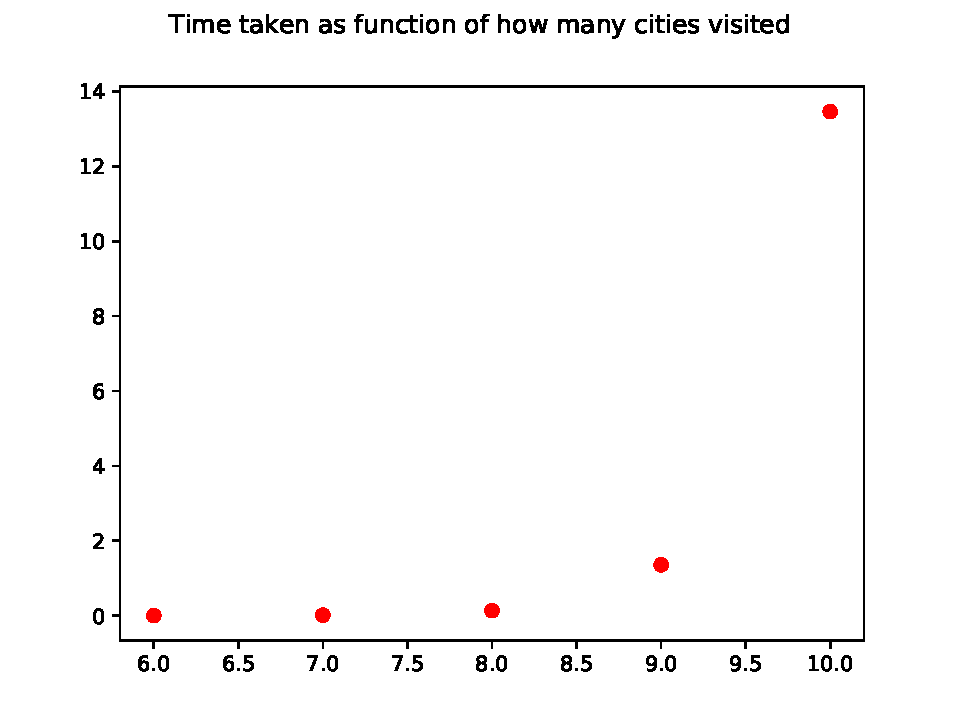
\includegraphics[scale=0.8]{"../Exhaustive.pdf}
\caption{Time spent for the TSP algorithm}
\end{center}
\end{figure}
\noindent
It can be seen that time spent by the algorithm searching for an optimal solution in TSP for  \textit{n} cities is roughly the time spent on searching for \textit{n-1} cities multiplied by \textit{n}. The time spent by the algorithm (on my laptop) to search for the optimal solution in TSP for 24 cities can be calculated with
\[
	t_{10} \frac{24!}{10!} \approx 14s \cdot \frac{24!}{10!} \approx 2.4 \cdot 10^{18}
\]
which is around 76 billion years.

\section{Hill Climbing}
This algorithm was made based on \cite[chapter 9.4.3]{marsland}. 
 
Start the program with
\begin{lstlisting}[language=bash]
	$ python3 hill_climber.py european_cities.csv 
\end{lstlisting}
The program will try to find the shortest route between 10 and the shortest route between 24 cities. The program outputs

\begin{lstlisting}[language=bash]
	For 10 cities:
	Running the algorithm 20 times
	Number of searches per round: 10000
	Best distance: 7503.099999999999
	Worst distance: 8324.82
	Average distance: 7835.56
	Standard deviation: 229.896
	Time taken per search[seconds]: 0.145487
 
	For 24 cities:
	Running the algorithm 20 times
	Number of searches per round: 10000
	Best distance: 19413.899999999998
	Worst distance: 22341.170000000006
	Average distance: 21236.6
	Standard deviation: 751.52
	Time taken per search[seconds]: 2.017303
\end{lstlisting}
\noindent
The best result of 20 hill climber runs gets close to the solution computed by the exhaustive search (7503 vs 7486). Results of 7486 have a been observed during test runs.

The hill climber uses 10000 iterations each run, using a total of 200000 iterations to find this result. The exhaustive search on the other hand uses 10! = 3628800 iterations.

Increasing the iterations used by the hill climber reduces the standard deviation and increases the chances of it finding the optimal distance.

When searching 24 cities, the hill climber uses around two seconds every run, resulting in a total of around 40 seconds for the whole run. This is in strong contrast to the 76 billion years of the exhaustive search. However, the result found is quite far from the optimal one, but gets better if number of iterations increases.

\section{Genetic algorithm}
This algorithm was made based on \cite[chapter 3 - 6]{eiben}. All in all, the algorithm consist of:
\begin{itemize}
\item An initializer: random permutations computed using numpy.
\item A parent selector: using a linear ranking scheme with \textit{s} = 1.5.
\item A crossover algorithm: cycle crossover.
\item A mutating scheme: inversion of subset of cities in the children. Probability of mutation: 50\%
\item Survivor selector: GENITOR. The \textit{n} weakest parents are replaced by \textit{n} children. I have chosen \textit{n} = 4 for all my runs.
\end{itemize}
\noindent
The program was tested with a population of 10, 50 and 100.

Start the program with
\begin{lstlisting}[language=bash]
	$ python3 genetic_algorithm.py european_cities.csv 
\end{lstlisting}
The program will try to find the shortest distance between 24 cities using the three different population sizes, and then do the same with 10 cities. The program outputs:
\begin{lstlisting}[language=bash]
	Search: 24 cities, population size: 10, number of generations: 500, 
	number of rounds: 20, number of children: 4: 
	Best distance: 13340.920000000002
	Worst distance: 17002.0
	Average distance: 15437.6
	Standard deviation: 851.065
	Time [seconds]: 4.982695
	Best order of travel: 
	Prague Berlin Warsaw Kiev Moscow Stockholm Saint Petersburg Hamburg Copenhagen 
	Dublin London Brussels Paris Madrid Barcelona Rome Milan Munich Belgrade 
	Istanbul Bucharest Sofia Budapest Vienna Prague
 
	Search: 24 cities, population size: 50, number of generations: 500, 
	number of rounds: 20, number of children: 4: 
	Best distance: 15607.64
	Worst distance: 19076.97
	Average distance: 17500.1
	Standard deviation: 839.583
	Time [seconds]: 10.528968
	Best order of travel: 
	Rome Milan Munich Budapest Prague Hamburg Copenhagen Stockholm Warsaw 
	Sofia Istanbul Bucharest Kiev Moscow Saint Petersburg Vienna Belgrade 
	Madrid Barcelona Paris Brussels Dublin London Berlin Rome
 
	Search: 24 cities, population size: 100, number of generations: 500, 
	number of rounds: 20, number of children: 4: 
	Best distance: 16469.68
	Worst distance: 21342.51
	Average distance: 19425.3
	Standard deviation: 1086.04
	Time [seconds]: 17.520685
	Best order of travel: 
	Budapest Kiev Moscow Stockholm Warsaw Saint Petersburg Prague Paris 
	Dublin Munich Rome Bucharest Belgrade Vienna Berlin Hamburg Copenhagen 
	Brussels London Milan Madrid Barcelona Sofia Istanbul Budapest
 
	Search: 10 cities, population size: 10, number of generations: 500, 
	number of rounds: 20, number of children: 4: 
	Best distance: 7486.309999999999
	Worst distance: 7503.1
	Average distance: 7490.51
	Standard deviation: 7.27028
	Time [seconds]: 2.610346
	Best order of travel: 
	Brussels Hamburg Copenhagen Berlin Budapest Bucharest Istanbul Belgrade 
	Barcelona Dublin Brussels
 
	Search: 10 cities, population size: 50, number of generations: 500, 
	number of rounds: 20, number of children: 4: 
	Best distance: 7486.309999999999
	Worst distance: 7663.510000000001
	Average distance: 7498.53
	Standard deviation: 38.433
	Time [seconds]: 6.380234
	Best order of travel: 
	Hamburg Brussels Dublin Barcelona Belgrade Istanbul Bucharest Budapest 
	Berlin Copenhagen Hamburg
 
	Search: 10 cities, population size: 50, number of generations: 500, 
	number of rounds: 20, number of children: 4: 
	Best distance: 7486.309999999999
	Worst distance: 7603.24
	Average distance: 7501.36
	Standard deviation: 34.5993
	Time [seconds]: 6.684515
	Best order of travel: 
	Belgrade Istanbul Bucharest Budapest Berlin Copenhagen Hamburg Brussels 
	Dublin Barcelona Belgrade
\end{lstlisting}
\noindent
A plot of the average fitness of the best individual of each generation can be seen in figure 2.
\begin{figure}[H]
\begin{center}
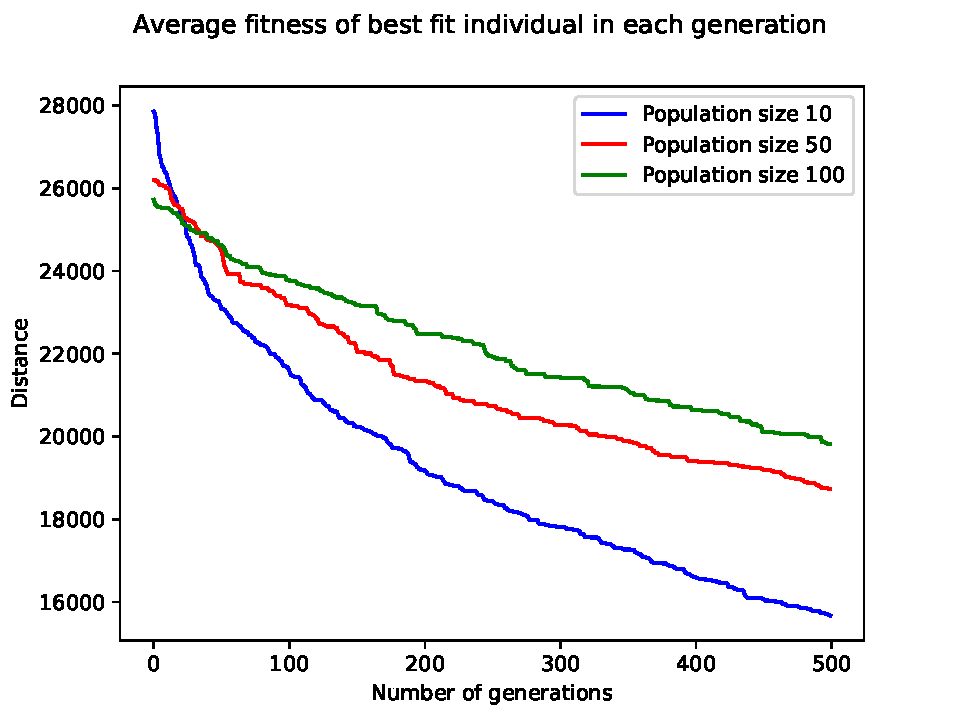
\includegraphics[scale=0.8]{"../genetic_algorithm.pdf}
\caption{Average fitness result for the genetic algorithm}
\end{center}
\end{figure}
\noindent
As shown in the plot and the output, the algorithm converges slower as population size increases. A reason for this might be because the survivor selection do not scale with the population size (\textit{n} = 4 for all population sizes). For this setup, the smaller population size (or the bigger ratio between \textit{n} and population size) gives the most effective and fruitful search.

The genetic algorithm is run 500 times, generating 500 generations of data. When looking at how the results from running the genetic algorithm with 10 cities compares with exhaustive search and hill climber, we see that it finds the optimal solution from exhaustive search, but using far less iterations that the hill climber,
\section{Hybrid algorithm}
The algorithm was made by modifying the genetic algorithm, adding a number of iterations of the hill climber to the parent selection. This was done by using the hill climber on every parent, then sorting the parents based on the new fitness values. For the Lamarckian learning model, the pre hill climb values were discarded and the new ones kept, while for the Baldwinian learning, the new fitness values were discarded amd the old ones kept. For this run I used hill climber with 3 iterations and the same population sizes as the genetic algorithm.

Start the program with
\begin{lstlisting}[language=bash]
	$ python3 hybrid_algorithm.py european_cities.csv 
\end{lstlisting}

\subsection{Lamarckian learning model}
The part of the programming testing the Lamrarckian learning model outputs:
\begin{lstlisting}[language=bash]
	---- LAMARCKIAN LEARNING MODEL ----
	Search: 24 cities, population size: 10, number of generations: 500, 
	number of rounds: 20, number of children: 4, 
	number of hill climb iterations: 3: 
	Best distance: 12384.219999999998
	Worst distance: 14111.69
	Average distance: 13115.3
	Standard deviation: 501.122
	Time [seconds]: 23.187871
	Best order of travel: 
	Moscow Saint Petersburg Stockholm Copenhagen Hamburg Dublin London Paris 
	Brussels Munich Milan Madrid Barcelona Rome Sofia Istanbul Bucharest 
	Belgrade Budapest Vienna Prague Berlin Warsaw Kiev Moscow
 
	Search: 24 cities, population size: 50, number of generations: 500, 
	number of rounds: 20, number of children: 4, 
	number of hill climb iterations: 3: 
	Best distance: 12384.22
	Worst distance: 13501.650000000001
	Average distance: 12900.0
	Standard deviation: 288.045
	Time [seconds]: 99.415685
	Best order of travel: 
	Moscow Kiev Bucharest Istanbul Sofia Belgrade Rome Milan Barcelona Madrid 
	Paris Dublin London Brussels Hamburg Copenhagen Stockholm Berlin Prague 
	Munich Vienna Budapest Warsaw Saint Petersburg Moscow
 
	Search: 24 cities, population size: 100, number of generations: 500, 
	number of rounds: 20, number of children: 4, 
	number of hill climb iterations: 3: 
	Best distance: 12325.930000000002
	Worst distance: 13476.589999999998
	Average distance: 12827.5
	Standard deviation: 275.802
	Time [seconds]: 199.236898
	Best order of travel: 
	Copenhagen Berlin Warsaw Stockholm Saint Petersburg Moscow Kiev Istanbul 
	Bucharest Sofia Belgrade Budapest Vienna Prague Munich Milan Rome Barcelona 
	Madrid Paris Brussels London Dublin Hamburg Copenhagen
 
	Search: 10 cities, population size: 10, number of generations: 500, 
	number of rounds: 20, number of children: 4, 
	number of hill climb iterations: 3: 
	Best distance: 7486.3099999999995
	Worst distance: 7503.099999999999
	Average distance: 7488.83
	Standard deviation: 5.99523
	Best order of travel: 
	Dublin Brussels Hamburg Copenhagen Berlin Budapest Bucharest Istanbul 
	Belgrade Barcelona Dublin
 
	Search: 10 cities, population size: 50, number of generations: 500, 
	number of rounds: 20, number of children: 4, 
	number of hill climb iterations: 3: 
	Best distance: 7486.309999999999
	Worst distance: 7486.3099999999995
	Average distance: 7486.31
	Standard deviation: 5.85938e-05
	Time [seconds]: 64.33309
	Best order of travel: 
	Hamburg Brussels Dublin Barcelona Belgrade Istanbul Bucharest Budapest 
	Berlin Copenhagen Hamburg
 
	Search: 10 cities, population size: 100, number of generations: 500, 
	number of rounds: 20, number of children: 4, 
	number of hill climb iterations: 3: 
	Best distance: 7486.309999999999
	Worst distance: 7486.3099999999995
	Average distance: 7486.31
	Standard deviation: 5.85938e-05
	Time [seconds]: 128.094541
	Best order of travel: 
	Istanbul Bucharest Budapest Berlin Copenhagen Hamburg Brussels Dublin 
	Barcelona Belgrade Istanbul
\end{lstlisting}
\noindent
A plot of the average fitness of the best individual of each generation can be seen in figure 3.
\begin{figure}[H]
\begin{center}
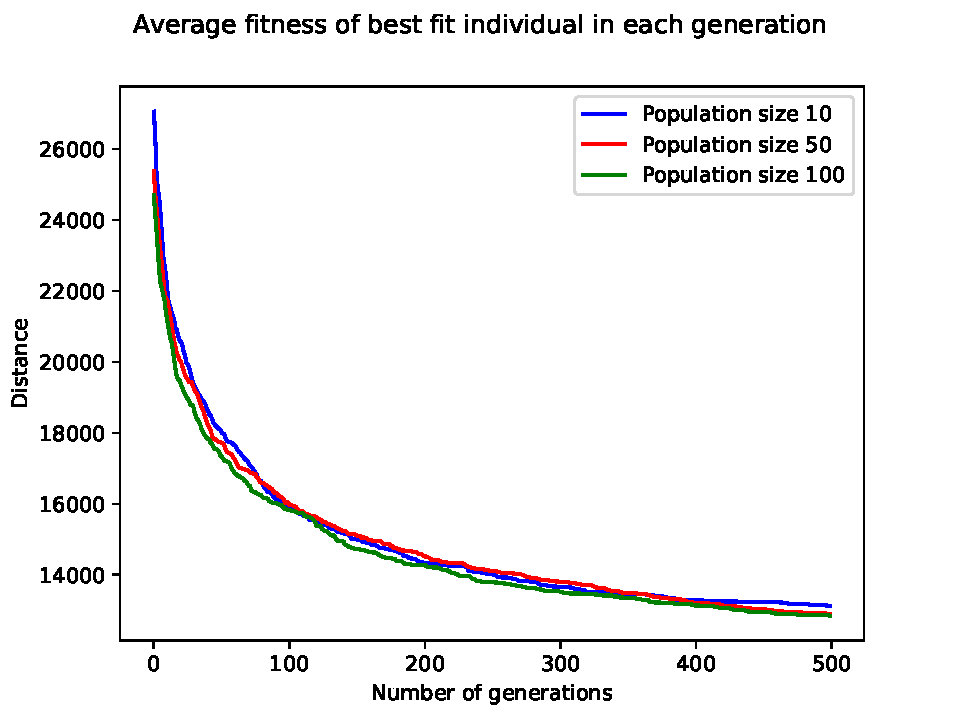
\includegraphics[scale=0.8]{"../hybrid_algorithm_lamarckian.pdf}
\caption{Average fitness result for the hybrid algorithm with a Lamarckian learning model}
\end{center}
\end{figure}
\noindent
As shown in the plot and the output, the algorithms converges faster than the genetic algorithm when using the same number of generations. The three populations converges approximately at the same speed. The standard deviation decreases as the population size increases.

\subsection{Baldwinian learning model}
The part of the programming testing the Baldwinian learning model outputs:
\begin{lstlisting}[language=bash]
	---- BALDWINIAN LEARNING MODEL ----
	Search: 24 cities, population size: 10, number of generations: 500, 
	number of rounds: 20, number of children: 4, 
	number of hill climb iterations: 3: 
	Best distance: 24573.85
	Worst distance: 33081.719999999994
	Average distance: 28469.5
	Standard deviation: 2413.0
	Time [seconds]: 28.799268
	Best order of travel: 
	Bucharest Istanbul Rome Dublin London Berlin Milan Prague Copenhagen 
	Warsaw Saint Petersburg Kiev Moscow Stockholm Vienna Brussels Paris 
	Munich Belgrade Sofia Barcelona Budapest Hamburg Madrid Bucharest
 
	Search: 24 cities, population size: 50, number of generations: 500, 
	number of rounds: 20, number of children: 4,
	number of hill climb iterations: 3: 
	Best distance: 22539.57
	Worst distance: 32637.84
	Average distance: 27822.1
	Standard deviation: 2372.2
	Time [seconds]: 131.015888
	Best order of travel: 
	Hamburg Stockholm Warsaw Munich Milan Madrid Budapest Kiev Moscow 
	Belgrade Istanbul Saint Petersburg London Berlin Sofia Vienna Rome 
	Brussels Bucharest Paris Dublin Barcelona Prague Copenhagen Hamburg
 
	Search: 24 cities, population size: 100, number of generations: 500, 
	number of rounds: 20, number of children: 4, 
	number of hill climb iterations: 3: 
	Best distance: 24413.59
	Worst distance: 31961.609999999993
	Average distance: 26829.1
	Standard deviation: 1923.99
	Time [seconds]: 268.707197
	Best order of travel: 
	Milan Madrid Copenhagen Stockholm Sofia Istanbul Hamburg Paris Prague 
	Berlin Saint Petersburg Moscow Warsaw Rome Vienna London Bucharest 
	Budapest Kiev Belgrade Brussels Munich Barcelona Dublin Milan
 
	Search: 10 cities, population size: 10, number of generations: 500, 
	number of rounds: 20, number of children: 4, 
	number of hill climb iterations: 3: 
	Best distance: 8895.97
	Worst distance: 14540.27
	Average distance: 11162.9
	Standard deviation: 1312.17
	Time [seconds]: 16.562146
	Best order of travel: 
	Brussels Belgrade Istanbul Bucharest Dublin Barcelona Budapest Hamburg 
	Copenhagen Berlin Brussels
 
	Search: 10 cities, population size: 50, number of generations: 500, 
	number of rounds: 20, number of children: 4, 
	number of hill climb iterations: 3: 
	Best distance: 8304.14
	Worst distance: 14255.750000000002
	Average distance: 10502.8
	Standard deviation: 1614.64
	Time [seconds]: 82.029157
	Best order of travel: 
	Brussels Dublin Barcelona Hamburg Istanbul Bucharest Belgrade Budapest 
	Berlin Copenhagen Brussels
 
	Search: 10 cities, population size: 100, number of generations: 500, 
	number of rounds: 20, number of children: 4, 
	number of hill climb iterations: 3: 
	Best distance: 8514.890000000001
	Worst distance: 14829.510000000002
	Average distance: 10811.2
	Standard deviation: 2013.73
	Time [seconds]: 159.45777
	Best order of travel: 
	Budapest Bucharest Dublin Belgrade Hamburg Istanbul Brussels Copenhagen 
	Berlin Barcelona Budapest

\end{lstlisting}
\noindent
A plot of the average fitness of the best individual of each generation can be seen in figure 4.
\begin{figure}[H]
\begin{center}
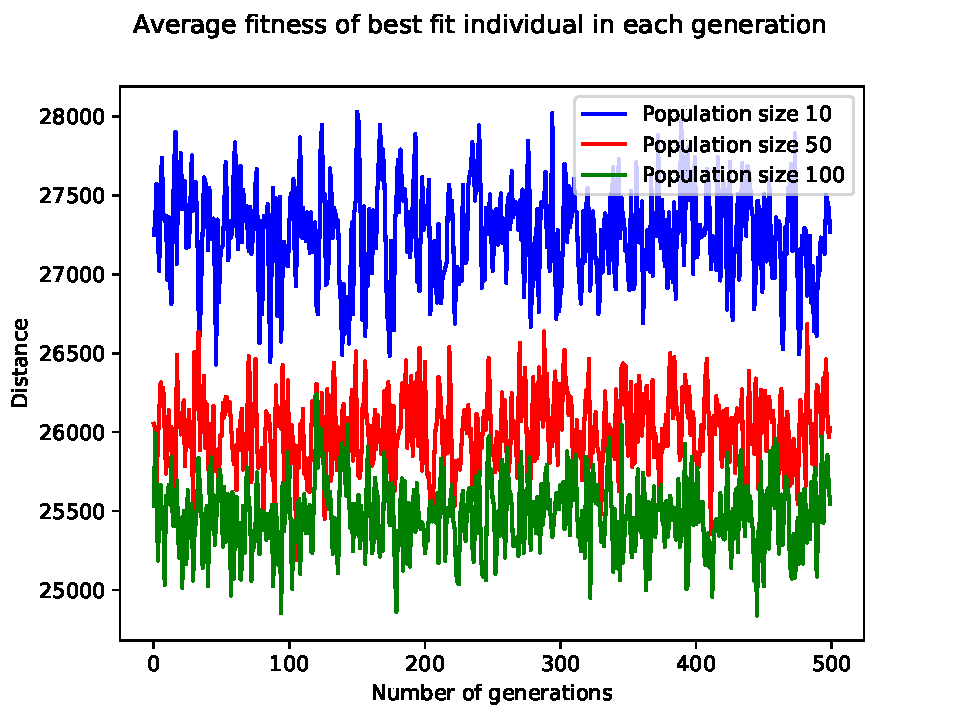
\includegraphics[scale=0.8]{"../hybrid_algorithm_baldwinian.pdf}
\caption{Average fitness result for the hybrid algorithm with a Baldwinian learning model}
\end{center}
\end{figure}
As shown in the plot and output, the Baldwinian learning model fails
\begin{thebibliography}{9}

\bibitem{eiben}
  A.E Eiben, J.E Smith,
  \textit{Introduction to Evolutionary Computing},
  Springer, London,
  2nd edition,
  2015.
  
\bibitem{marsland}
  Stephen Marsland,
  \textit{Machine Learning - An Algorithmic Perspective},
  Chapman and Hall/CRC, Boca Raton/London/New York,
  2nd edition,
  2015.

\end{thebibliography}

\end{document}
